\section{Virtual Group Room} %hej kim
\label{sec:projGroupRoomImpl}
In this section the actual implementation of the virtual group room, its custom blocks, and the navigation to the project groups of the users is described. %% This sentence is dedicated to Miral. GLHF!!
%The section presents how the project groups work from the perspective of the user. 



%The task of securing that only members of the project group can edit and view are maintained by the project group room and is described in \secref{sec:projectgrouproommanagerights}. 


\subsection{Blocks}
\label{sec:implprojectgroupblocks}
\label{sub:membersblock}
When a new project group is created a number of default blocks are added to the virtual group room. 
The default blocks are specified in a configuration file, \moodlefile{/local/projectgroup/config.php}, and the content can be seen in \coderef{moodledaultblock}


\begin{lstlisting}[style=phpCode, caption=\myCaption{The default block configuration}, label=moodledaultblock]
<?php
	/**
	* Example usage:
	* "left1,left2:center1:right1"
	* Will add two items to the left, one in the middle, and one to the right
	*/
	$format['defaultprojectgroupblocks'] = ':projectgroup_members,timeline,groupwall,blackboard:upload,tasks';
\end{lstlisting}\begin{comment}$\end{comment}
The syntax for the format is \verb{left:middle:right{. 
Left, middle, and right represent the three columns in the virtual group room. 
The blocks Timeline, groupwall, blackboard, upload, and tasks are created by our peer-groups while the block named projectgroup\_members is created by us. 

As described in \secref{sec:requirements} the projectgroup\_members block shows the names and photographs of the project group members. 
It is implemented as a \block{} in the same manner as the \block{}s created by our peer-groups, although our \block{} is less complicated. 
All it does is fetching the members of the project group using the function \fu{get\_projectgroup\_members} and presenting these along with a photograph for each member, which is fetched through a Moodle API call. 

The layout of a virtual group room can be seen on \figref{fig:projectgroupnoedit} in \chapref{sub:page}.





\subsection{Navigation}
\label{sub:navimpl}
%In \secref{sub:designprojectgroupnavigation} the navigation to project groups is described and in this section the actual implantation of the navigation described. 
From \secref{sec:requirements} we have a requirement called \req{Navigate to Project Groups} which states that a user should be able to find the project group(s) that he is a member of.
This implementation that satisfies this requirement is presented here.
Since we implement the virtual group room as a local plugin we can use a built-in functionality of \moodle{} to extend the navigation block~\cite{moodleextendnavigationblock}.
The navigation menu can be seen in \figref{fig:moodlenavigationblock}.
The extended part is highlighted by the rectangle. 

\begin{figure}
	\centering
		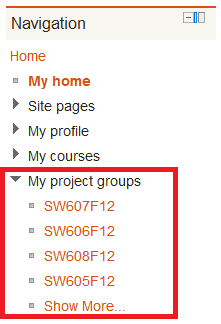
\includegraphics[scale=0.7]{images/moodlenavigationblock.png}
		\morscaption{Navigation block. The highlighted box shows our extension with a list of project groups, which the currently logged in user is a member of}
	\label{fig:moodlenavigationblock}
\end{figure}

The code to add project groups to the navigation block can be seen in \coderef{src:moodlecodeextendingnavigation}.
The currently logged in user is accessed to get the project groups that he is a member of.
The code checks if something should be displayed at all and then run a loop to print out the link to each group. 
If more than four project groups is associate with the given user a link to ``Show More'' is added and no more links are generated.
This link takes the user to an overview showing all project groups that he is a members of.


\begin{lstlisting}[style=phpCode, caption=\myCaption{The code for extending the navigation block}, label=src:moodlecodeextendingnavigation]
function projectgroup_extends_navigation(global_navigation $navigation) 
{
	global $USER;
	$number_of_groups = 4;
	
	...
	
	$groups = get_groups_of_user($USER->id);
	if(sizeof($groups) > 0)
	{
		$type = navigation_node::TYPE_CUSTOM;
		$my_projectgroup_navigation = $navigation->add(get_string('myprojectgroup','local_projectgroup'),null,$type,null,'myprojectgroup');
		$count = 0;
		foreach ($groups as $group_id) 
		{
			$count++;
			if($count > $number_of_groups ){
				$my_projectgroup_navigation->add('Show More...', 
					new moodle_url('/local/projectgroup/usergroups.php',
					array('id'=>$USER->id, 'sesskey'=>sesskey())),
					$type,null,'show_more');
				break;
			}
			$group = get_projectgroup($group_id);
			$my_projectgroup_navigation->add($group->shortname, new moodle_url('/local/projectgroup/index.php', array('id'=>$group_id, 'sesskey'=>sesskey())),$type,null,$group->id);
			
		}
	}
}
\end{lstlisting}












